\chapter{System Analysis}

The project hosts two kinds of roles: admins and users. 

The user will start a trip, save location and media, manipulate media share options and share all of contents on social media. Also user can download a shared content which that user has access privileges. User can follow the trip that downloaded. User can search other users; trips by location, name and trip type (walk, run, ride or car). User can organize team trips with other users. During the team trip users can see each other's location on the map.

The admins can view the content of trips or profile of users. They can also evaluate the complaints which has been created by users. They can decide whether they are right or not, if admins think the complaint that is created by users is right they can hide the content of profile,comment or the whole trip. They are also able to view the support messages. 

The work model of the system is shown in Figure~\ref{fig:system_diagram}, user roles shown in Figure \ref{fig:roles} and used technologies shown in Figure \ref{fig:usedTechnologies}. Workflow schema for creating a personal trip shown in Figure \ref{fig:personalTripWorkflow} and workflow schema for creating a team trip shown in Figure \ref{fig:teamTripWorkflow}. 

\begin{figure}[!htbp]
\centering
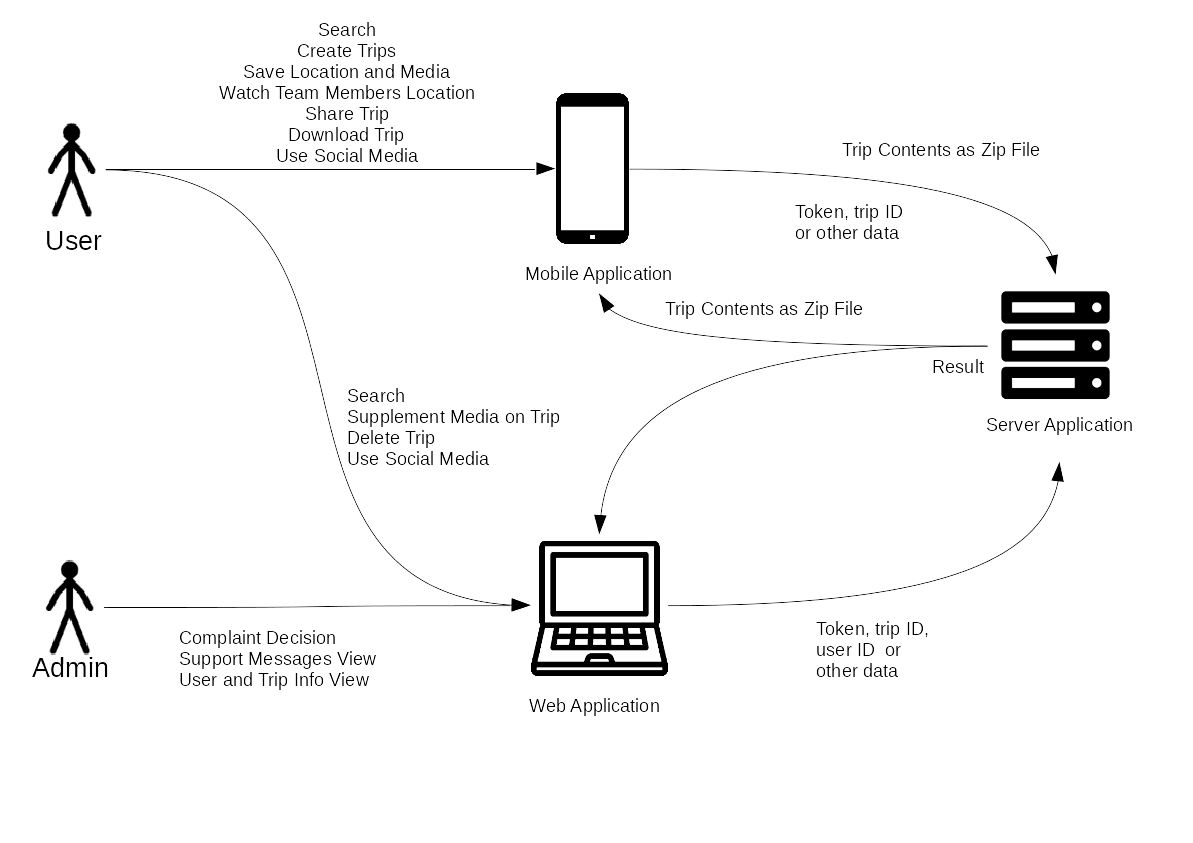
\includegraphics[width=\textwidth]{projectChapters/images/system_diagram.png}
\caption{System Schema}
\label{fig:system_diagram}
\end{figure}

\begin{figure}[!htbp]
\centering
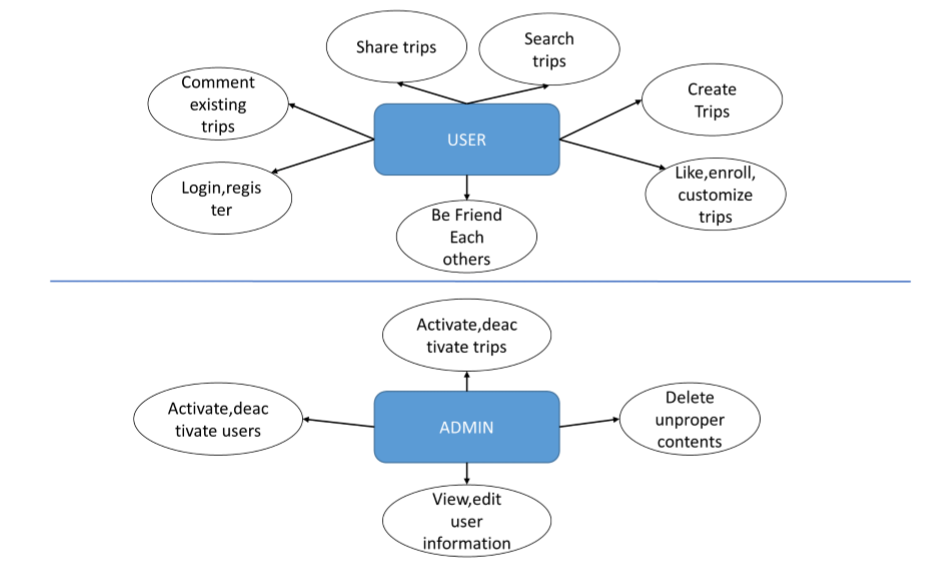
\includegraphics[width=\textwidth]{projectChapters/images/ER.png}
\caption{User Roles}
\label{fig:roles}
\end{figure}

\begin{figure}[!htbp]
\centering
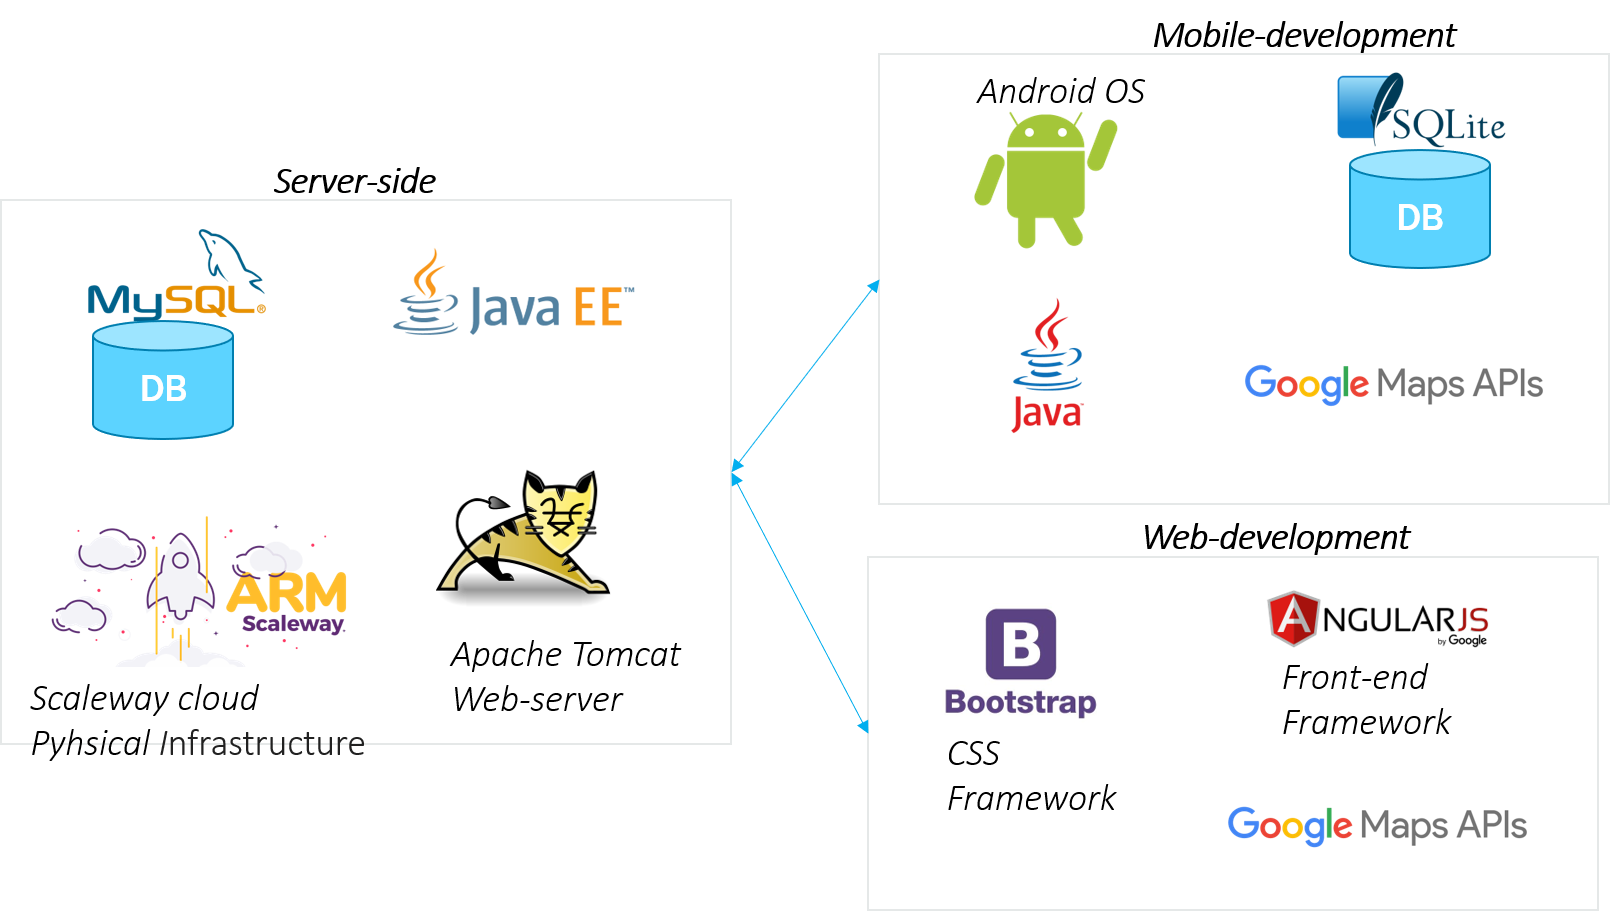
\includegraphics[width=\textwidth]{projectChapters/images/usedTechnologies.png}
\caption{Used Technologies}
\label{fig:usedTechnologies}
\end{figure}

\begin{figure}[!htbp]
\centering
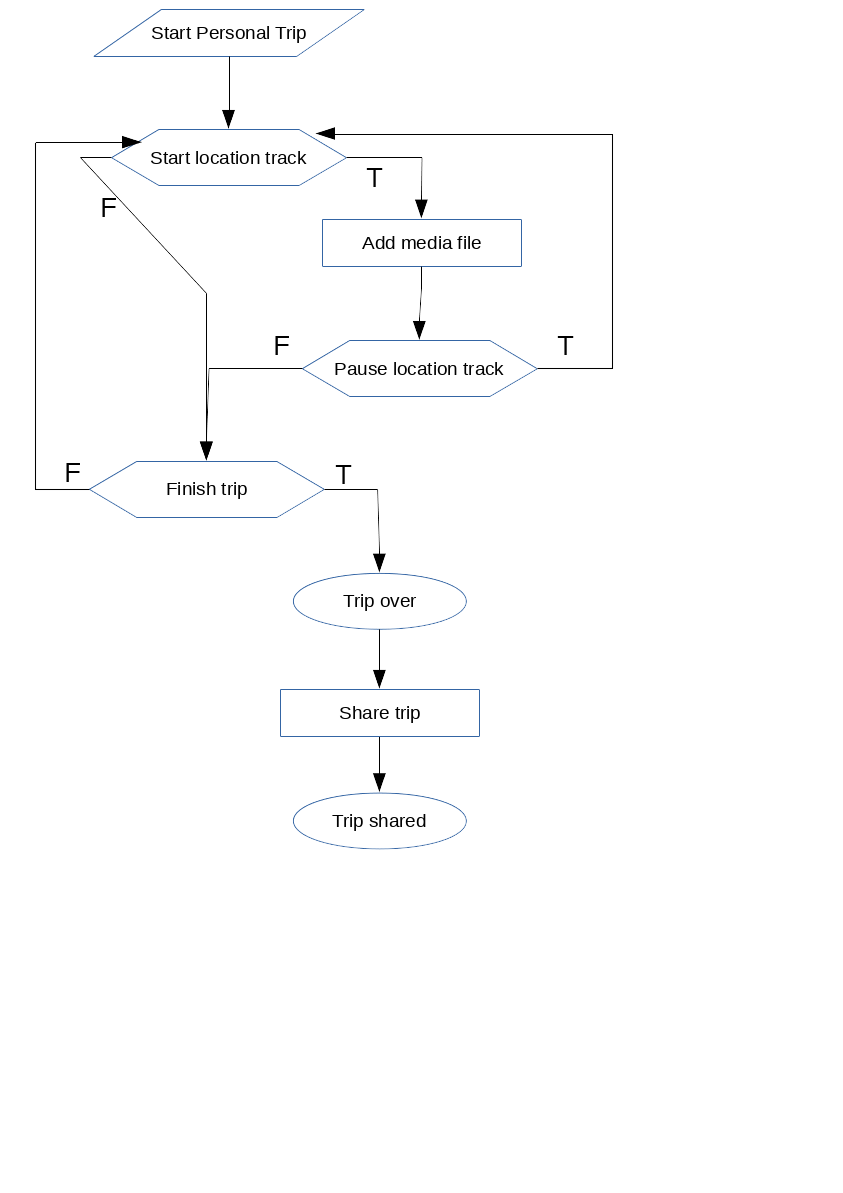
\includegraphics[width=\textwidth]{projectChapters/images/personalTripWorkflow.png}
\caption{Workflow Schema For Creating Personal Trip}
\label{fig:personalTripWorkflow}
\end{figure}

\begin{figure}[!htbp]
\centering
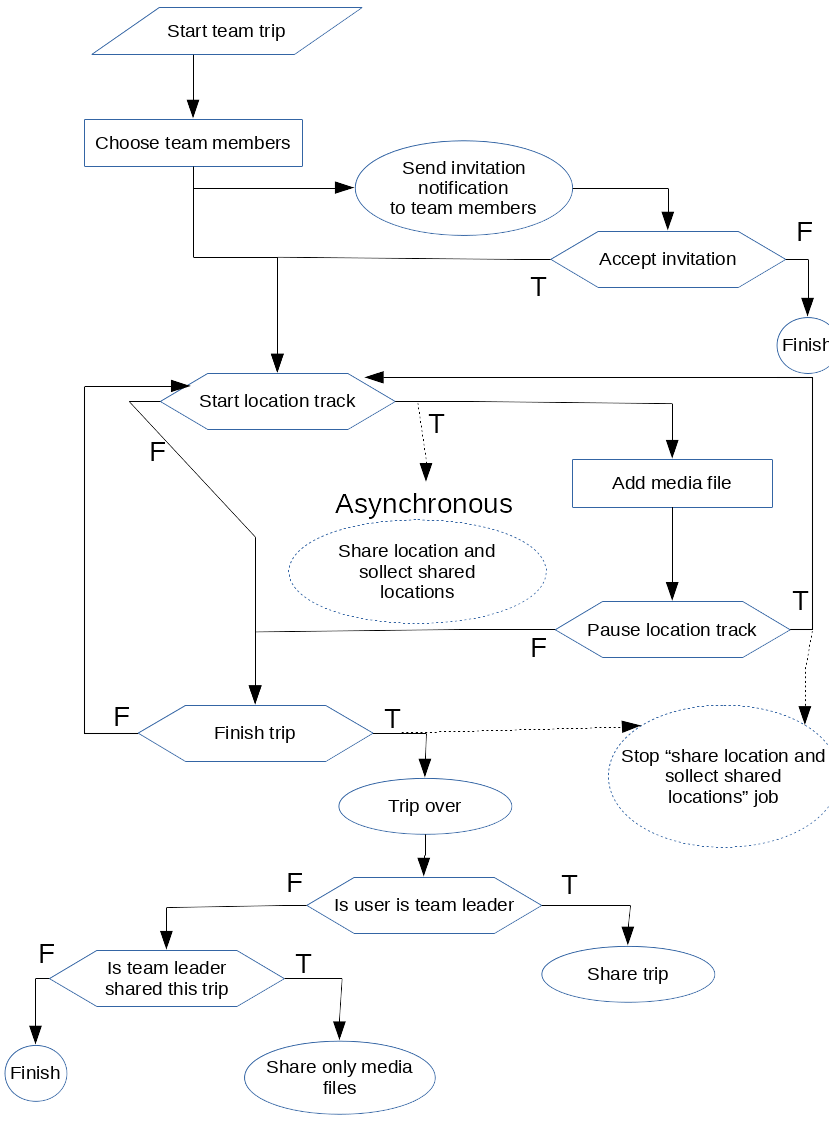
\includegraphics[width=\textwidth]{projectChapters/images/teamTripWorkflow.png}
\caption{Workflow Schema For Creating Team Trip}
\label{fig:teamTripWorkflow}
\end{figure}